 \documentclass[journal]{IEEEtran}
\interdisplaylinepenalty=2500

\usepackage{array}
\usepackage{graphicx}
\usepackage{epsf}
\usepackage{float}
\usepackage{stfloats}
\usepackage[font=footnotesize]{caption}
\usepackage[font=footnotesize]{subcaption}
\usepackage{cite}
\usepackage{picinpar}
\usepackage{siunitx}

\usepackage{amsmath, nccmath}
\usepackage{url}
\usepackage{flushend}
\usepackage{colortbl}
\usepackage{soul}
\usepackage{multirow}
\usepackage{pifont}
\usepackage{color}
\usepackage{alltt}
\usepackage[hidelinks]{hyperref}
\usepackage{enumerate}
\usepackage{siunitx}
\usepackage{breakurl}
\usepackage{epstopdf}
\usepackage{pbox}


\usepackage{booktabs}
\usepackage{wrapfig}

\graphicspath{{../}}

\usepackage{placeins}
\usepackage{latexsym}
\usepackage{amssymb}
\usepackage{xifthen}
\usepackage{balance}
\usepackage{multicol}
\renewcommand{\arraystretch}{1.2}




\newenvironment{conditions}
  {\par\vspace{\abovedisplayskip}\noindent\begin{tabular}{>{$}l<{$} @{${}-{}$} l}}
  {\end{tabular}\par\vspace{\belowdisplayskip}}


\ifCLASSINFOpdf

\else
 
\fi


\hyphenation{op-tical net-works semi-conduc-tor}


\begin{document}

\title{Analysis and Implementation of Multisampled PWM for High Bandwidth and Output Frequency Current Control of Electrical Drives}

\author{
	\vskip 1em
	{
	Ivan Z. Petric, \emph{Student Member, IEEE},
	Ruzica Cvetanovic,
	}
}


% make the title area
\maketitle

\begin{abstract}
This paper investigates a nonlinear phenomenon related to multisampling control of power converters. The nonlinearity, manifested as increased gain regions in static modulator transcharacteristic, is caused by the discontinuity of the modulating waveform, and can result in increased jittering of the duty-cycle. The paper proposes a statistical model for predicting the jittering impact on the duty cycle variance, analytic derivations for the jittering conditions, and an anti-jittering algorithm. An analytically obtained static modulator transcharacteristic is given to illustrate the increased gain regions.
Verifications, performed on a multisampled digitally controlled buck converter, show a good match between the theoretical analysis, simulations and experimental results. This paper is accompanied by videos demonstrating the jitter amplification and the algorithm operation.
\end{abstract}

% Note that keywords are not normally used for peerreview papers.
\begin{IEEEkeywords}
Digital pulse-width modulators (DPWM), Jittering, Limit-cycle oscillations (LCOs), Multisampled pulse-width modulators (MS-PWM) 
\end{IEEEkeywords}


\IEEEpeerreviewmaketitle

\section{Introduction}
\IEEEPARstart{F}{ield} oriented control (FOC) is a well-established strategy for the control of high performance electrical drives \cite{holmes2012}. An essential part of this concept is the inner current control loop \cite{holmes2009}. A prerequisite for the proper operation of the outer control loops is a precise and rapid digital current controller \cite{yepes2014}. In order to achieve the desirable performance of the overall control system high current loop bandwidth is imperative \cite{choi1998}. Robustness at high output frequencies, along with a decoupled d and q axis transient operation is also required ~\cite{choi1998,hoffmann2016,yim2009}. Digital control introduces delays due to the sampling process, execution time and digital pulse width modulation (DPWM) \cite{holmes2009}. These delays limit the achievable bandwidths and motivate the direct discrete-time domain design of high-performance current controllers \cite{bae2003}. These limitations have inspired investigating multisampled PWM control, with purpose of enabling analog-like control bandwidths in digital systems. The multisampling approach relies on acquiring the control variables and updating the modulating waveform multiple times per switching period \cite{corradini_analysis}. The concept of multisampled digital control offers significant reduction of the modulator delays and therefore is a promising solution for breaking the bandwidth limitations \cite{corradini2018}. Besides improvements in dynamic perofrmance, MS-PWM is also reported to have a positive impact on the noise attenuation \cite{petric2020}. 

Synchronous rotating frame (SRF) PI controllers are the most frequently encountered current control concepts since they are simple and successfully cover the majority of the industry requirements ~\cite{rowan1986,bae2003,yepes2014}. With a proper parameter setting procedure, high bandwidths can be achieved ~\cite{yepes2014,holmes2009}. Nevertheless, their transient decoupling capability is rather limited, especially at high speeds \cite{lorenz2000}. On the other hand, model predictive dead-beat current controllers offer very fast transient response but at the cost of considerable performance degradation when parameter mismatch occurs ~\cite{malesani1999,xu2019}. Since saturation and temperature variations are very often encountered in electrical drives, a simple dead-beat approach might lead to insufficient performance. An FPGA implementation of the robust multisampled dead-beat control has been proposed in \cite{rovere2018}. Another promising current control approach is the discrete internal model principle (IMC) design \cite{lorenz2010}. Since no S domain based delay approximations are used, axes cross-coupling is inherently eliminated and high closed loop bandwidths can be achieved ~\cite{commentsHoffmann,vuksa2016}. Despite all of the benefits of feedback averaging, the addition of a moving average filter in feedback path can considerably degrade the performance of the current control loop \cite{vuksa2016}. The IMC concept however, with some enhancements of the controller structure in terms of addition of differential compensator and advanced scheduling scheme, achieves very fast and robust current tracking even with MAF in the feedback path \cite{vuksa2017}. Further improvements in terms of active resistance feedback result in high disturbance rejection capability \cite{vuksa2018}. 

This paper analyzes the use of MS-PWM in discrete IMC based current controller, suitable for implementation on standard DSP platforms. The main goal of the paper is to demonstrate a current control structure, which offers improved dynamic response and high noise suppression compared to the state-of-the-art double update rate solutions. This is achieved without relying on expensive and complicated control platforms, but on a standard industrial DSP. The MS-PWM control strategy is analyzed for three different control loop organizations. The first one uses discrete IMC controller from \cite{vuksa2016}, with a moving average filter (MAF) in the feedback. This case is found to offer slightly improved dynamics compared to standard use of double-update with the same discrete IMC (without filter in feedback) ~\cite{lorenz2010,vuksa2016}, with significant improvement in jitter suppression. Due to added delays introduced by the MAF, the second case adds a derivative action to the controller structure, as in \cite{vuksa2016}. This case is given to demonstrate that MS-PWM can offer even better dynamics than reported in \cite{vuksa2016}. The final case implements MS-PWM based discrete IMC, without any filters in feedback. This case is expected to provide the best dynamics, using discrete IMC without derivative gain. The feedback quality is expected to worsen compared to cases with MAFs, hower, it still retains higher quality compared to double-update \cite{petric2020}. The target is to show that with the multisampling approach delays introduced by feedback averaging can be successfully compensated, by extent determined with the multisampling factor, enabling both robust and error-free feedback acquisition and a high dynamic performance of the current loop.

This paper is organized as follows. Section II addresses discrete time machine model, controller structure and analyzes delays introduced by feedback averaging, calculation and DPWM. The multisampling PWM approach, with an outline of its merits and demerits, is explained in Section III. A DSP implementation of the multisampling algorithm is also presented. Exact controller structures and parameter setting procedures for the three aforementioned cases of interest are derived in Section IV. Effectiveness of the derived analytical model is illustrated via simulated current loop step responses and frequency response analyses. Comparison between performance of the proposed methodology and benchmark controllers is also provided. Experimental results are shown in section V. Conclusions are drawn in section VI, along with a proposal for further studies on the presented topic.
 
\section{Machine model and control loop}

\subsection{Multisampled control stage of a buck converter}

\begin{figure}[t!]
    \centerline{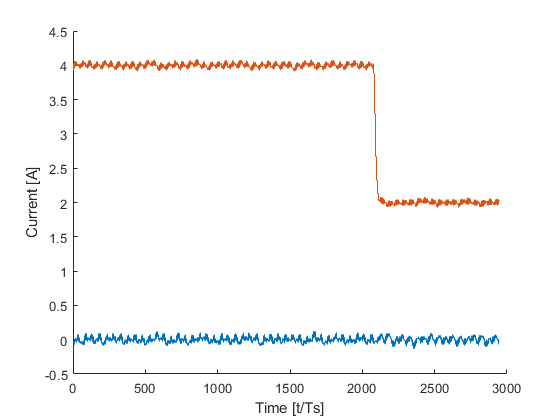
\includegraphics[width=0.95\linewidth]{figures/nas_step.png}}
    \caption{Multisampled control loop of a buck converter.}
    \label{fig:MSControl}
\end{figure}

The block diagram of a buck power converter with a multisampled current control loop is shown in Fig. \ref{fig:MSControl}. The power stage and the sensing circuit are shown in blue color, representing continuous-time domain. The sensing circuit often comprises an analog low-pass filter (ALPF), which is used to reduce the aliasing effect. After the inductor current $i_L(t)$ is processed in the analog domain, it is sampled by the ADC resulting in a digital signal $i_{L,s}[k]$. Blocks shown in black color represent the digital part of the system, operating with frequency equal to $f_s = N f_{sw}$, where $N$ is the multisampling factor and $f_{sw}$ is the switching frequency of the converter. The digital system consists of an ADC, a digital feedback filter (DLPF) $G_{fb}(z)$, and a controller $G_c(z)$. A digital filter can help reduce the nonlinearities introduced by the DPWM in MS-PWM control. The controller outputs a digital modulating impulse train $m[k]$, which is kept constant as a modulating segment throughout the entire sampling period $T_s = \frac{1}{f_s}$. This zero-order hold (ZOH) action transforms $m[k]$ into a piecewise constant modulating waveform $m_h (t)$, which is compared with the carrier $w(t)$ inside the DPWM block. The symmetrical carrier is chosen due to its favorable characteristics in MS-PWM control. The segment of the carrier with a positive slope is defined as up-count and the segment with a negative slope is defined as a down-count. The output of the DPWM is a gate signal, labeled as $x(t)$.

For two-level MS-PWM converters, switching ripple is always introduced in the feedback signal. The difference between consecutive segments of the modulating waveform is determined by $T_s$, controller design, and switching ripple magnitude. This discontinuity leads to many unfavorable characteristics of the MS-PWM control, one of which is the jitter amplification described in this paper.
% zasto current loop
The analysis of the jitter amplification is focused on the current control loop as even in voltage controlled systems, for most applications, the inner current loop is employed. The jitter amplification mechanism itself is not expected to change for single-stage voltage loops, which is under investigation.

\subsection{Definitions}
For further analytic considerations, the duty cycle $D$ of the converter is defined as a sum of the up-count duty cycle $D_u$ and the down-count duty cycle $D_d$:
\begin{equation}
\begin{aligned}
D = D_u + D_d = \frac{\Delta t_{on,u}}{T_{sw}} + \frac{\Delta t_{on,d}}{T_{sw}},
\label{eq:duty_cycle_def} 
\end{aligned}    
\end{equation}
where $\Delta t_{on,u}$ is the switch on-time during the up-count, $\Delta t_{on,d}$ is the switch on-time during the down-count, and $T_{sw}$ is the carrier period. These variables, $D_u$ and $D_d$, are referred to as the \textbf{partial duty cycles}.
In case of horizontal crossings between $m_h(t)$ and $w(t)$, the duty cycle can also be expressed using values of modulating segments that first intersect with the carrier during up-count ($m_{off}$) and during down-count ($m_{on}$):
\begin{equation}
\begin{aligned}
D = \frac{m_{on}+m_{off}}{2}
\label{eq:duty_cycle_def_m} 
\end{aligned}    
\end{equation}

% in phase counter phase
The following definitions for possible relations between the modulating waveform $m_h(t)$ and the carrier $w(t)$ are introduced:

\begin{figure}[t!]
    \centerline{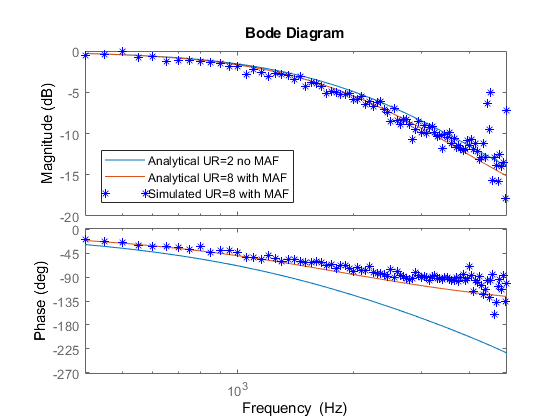
\includegraphics[width=0.95\linewidth]{figures/nas_clfra.png}}
    \caption{Modulating signal $m_h(t)$ and carrier $w(t)$ with a) counter-phase and b) in-phase operation.}
    \label{fig:InCounterPhase}
\end{figure}

\noindent
\begin{itemize}
\item{The \textbf{counter-phase} operation is shown in Fig. \ref{fig:InCounterPhase} a). During the carrier up-count, it occurs when, at the update instant of $m_h(t)$, closest to the intersection with $w(t)$, the value of $m_h(t)$ is decreased. During the carrier down-count, counter-phase operation occurs when at the closest update instant, $m_h(t)$ is increased. In Fig. \ref{fig:InCounterPhase}, the intersection is labeled with a red circle and the closest modulating signal update with a blue circle. 
For current loops without any feedback filtering, this regime is enabled by default due to the relation between the current ripple and the PWM output. This kind of operation can result in a nonlinear behaviour of MS-PWM caused by the vertical crossing of $m_h(t)$ with $w(t)$.}

\item{The \textbf{in-phase} operation is shown in Fig. \ref{fig:InCounterPhase} b). During the carrier up-count, it occurs when, at the update instant of $m_h(t)$, closest to the intersection with $w(t)$, the value of $m_h(t)$ is increased. During the carrier down-count, in-phase operation occurs when at the closest update instant, $m_h(t)$ is decreased. For current loops, this regime is enabled by feedback filtering that causes phase lag of the switching ripple component. The in-phase condition is necessary for the jitter amplification. The in-phase operating conditions for current loops are derived in subsection III B. Additionally, in-phase operation can be found without filtering in multilevel converters with phase-shifted carriers, as well as in voltage loops.}

\item{The \textbf{critical partial duty cycle} $D_c$ defines the operating point for which the modulating signal update may cause the jitter amplification. 
For a single carrier PWM modulation, the jittering can occur only for $D_u \approx D_c$ or $D_d \approx D_c$. Values of $D_c$ depend on the multisampling factor:
\begin{equation}
\begin{aligned}
D_c = \frac{k}{N} \quad , \quad 1 \leq k < \frac{N}{2} \label{eq:duty_crit} 
\end{aligned}    
\end{equation}
where $k$ is an integer that limits $D_c$ in the open interval $\left(0,\frac{1}{2} \right)$. 
It is evident that as $N$ increases, there are more critical partial duty cycles, but also the discontinuity of the modulating waveform decreases, which is why this paper focuses on $N \in \{ 4,6,8 \}$.}

\item{The \textbf{critical modulating segments} are a pair of subsequent segments that participate in the jitter amplification. For those, it is important to verify whether the in-phase regime is occurring. Depending on $D_c$ and $N$, the critical modulating segments are labelled as $m_{N , D_c \cdot N + n}$, where $n \in \{ 0,1 \}$. For example, for $N = 8$ and $D_c = \frac{1}{4}$ critical segments are $m_{8,2}$ and $m_{8,3}$}.
\end{itemize}

In Fig. \ref{fig:CriticalDuties}, modulating waveforms are shown for $N\in \left\lbrace 4,6,8 \right\rbrace$, for $D_u$ equal to the corresponding lowest value of $D_c$.

\begin{figure}[t!]
    \centerline{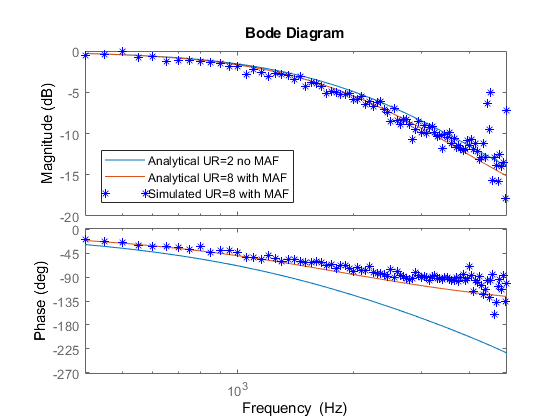
\includegraphics[width=0.95\linewidth]{figures/nas_clfra.png}}
    \caption{Critical duty cycles for $N \in \{4,6,8 \}$, for carrier up-count mode. }
    \label{fig:CriticalDuties}
\end{figure}

\subsection{Explanation of the jittering mechanism}

The jitter amplification phenomenon, described in this paper, is a result of the in-phase operation and the discontinuity of $m_h(t)$. The mechanism behind it is illustrated in Fig. \ref{fig:InPhaseJittering}, for $N = 4$ and $D_u \approx D_c = \frac{1}{4}$.
At operating points close to the critical partial duty cycles, switching action occurs near the instant at which $m_h(t)$ is updated. For in-phase operation, this update can cause another vertical intersection of $m_h(t)$ and $w(t)$, which can then cause an additional PWM output pulse. This is normally prevented by limiting the switching actions to a single turn-off for the carrier up-count, based on the first intersection between $m_h(t)$ and $w(t)$, and to a single turn-on for the carrier down-count. However, this condition can still lead to the jitter amplification.

Consider initial operating point, shown in Fig. \ref{fig:InPhaseJittering}, where intersection with the carrier during up-count occurs during modulating segment $m_{4,1}$. This results in duty cycle equal to $D_d + D_{u,1}$. With small-signal change of the controller output, such that higher duty cycle is required (value between $D_{d}+D_{u,1}$ and $D_{d}+D_{u,2}$), the modulating segment $m_{4,1}$ exhibits small-signal change in positive direction. As illustrated in Fig. \ref{fig:InPhaseJittering}, a very small positive change of the segment $m_{4,1}$ causes the intersection with $w(t)$ to occur during the following segment $m_{4,2}$, which changes the up-count duty cycle from $D_{u,1}$ to $D_{u,2}$. Since the applied up-count duty cycle is higher than required one, the controller will react by causing a negative change of $m_{4,1}$, which will again result in that segment causing intersection with $w(t)$. Hence, jittering occurs by extent that is determined by the discontinuity of $m_h(t)$:  $D = f (m_{4,2} - m_{4,1} , t)$. Depending on the controller, output ripple, $N$ and $T_s$, the critical modulating segments can feature significantly different values, which results in very high gain of the MS-PWM modulator - $\frac{\partial D}{\partial m_{4,1}}$. The incapability of MS-PWM modulator to achieve desired duty-cycle is manifested as "increased gain" regions in the modulator static transcharacteristic, which is given in subsection III C.

\begin{figure}[t!]
    \centerline{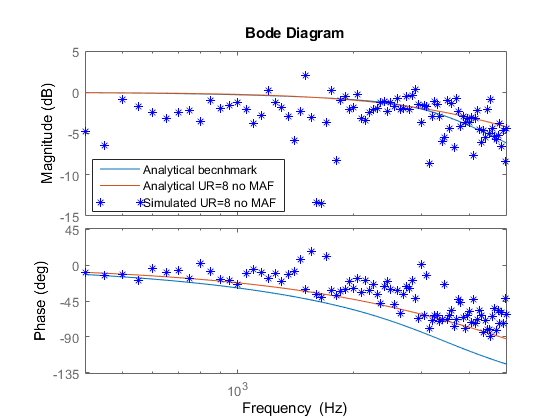
\includegraphics[width=0.95\linewidth]{figures/nasb_clfra.png}}
    \caption{Example of the jitter amplification for $N = 4$, $D_u \approx D_c = \frac{1}{4}$.}
    \label{fig:InPhaseJittering}
\end{figure}

Whether or not the in-phase operation occurs for a current control loop, depending on feedback filter, controller gains, multisampling factor and critical partial duty cycle is analytically derived in subsection III B. 

\section{MS-PWM approach}
In this section, a statistical approach is used to model the impact of the added jittering to the applied duty cycle. Subsequently, in-phase operating conditions are derived for current loops. In the end, the modulator static transcharacteristic is shown, in order to illustrate zones that cause jitter amplification.

\subsection{Statistical approach for jitter modelling}
In this subsection, a simple statistical approach is used to gain quantitative insight into the effect the jittering imposes on the converter output.
The principle behind the described effect is that a slight change of the modulating segment can lead to a big change of the switching pulse width.
In Fig. \ref{fig:InPhaseJittering}, the mechanism is shown for the jittering in the falling edge of the switching impulse, but it can equally appear for the rising edge or for both the edges. The equations are derived for the jittering of a single edge, based on the difference between values of the critical modulating segments.

Consider operating condition shown in Fig. \ref{fig:InPhaseJittering}. Assuming that the rising edge of the switching impulse is fixed (corresponding value of the modulating segment is $m_{on}$), the applied duty cycle depends on the value of the critical modulating segment that first intersects with the carrier during up-count. For a certain critical partial duty cycle, the critical modulating segments are $m_{N , D_c \cdot N}$ and $m_{N , D_c \cdot N + 1}$, which result in up-count duty-cycles equal to $D_{u,1}$ and $D_{u,2}$, respectively. Assuming that the required up-count duty-cycle is exactly in between of $D_{u,1}$ and $D_{u,2}$, it can be considered that there is an equal probability that the switching will occur at $t_{off,1}$, producing duty cycle $D_1$ or at $t_{off,2}$, producing duty cycle $D_2$. Hence, the expected value of the applied duty cycle $\mu_D$ is equal to:

\begin{equation}
\begin{aligned}
\mu_D = \frac{1}{2} \left(D_1 + D_2 \right) = \frac{1}{2} \left(m_{on} +  \frac{ m_{N , D_c \cdot N} + m_{N , D_c \cdot N + 1}}{2}\right) \label{eq:expected_D} 
\end{aligned}    
\end{equation}

\noindent
The variance of the applied duty cycle $ \sigma ^2 _D$ is calculated as:

\begin{equation}
\begin{aligned}
 \sigma ^2 _D = \frac{1}{2} \left( \left( D_1 - \mu _D \right)^2 + \left( D_2 - \mu _D  \right)^2 \right)
= \frac{\Delta m^2 }{16},	\label{eq:variance_D} 
\end{aligned}    
\end{equation}
where $\Delta m = m_{N , D_c \cdot N + 1} - m_{N , D_c \cdot N}$.
\noindent
The equation \eqref{eq:variance_D} gives insight that the variance of the duty cycle changes as a quadratic function of the difference between critical modulating segments. Therefore, the reduction of the modulating waveform discontinuity strongly reduces the negative effect on the converter output. Note that for jittering during both up- and down-count regimes, the total variance is equal to sum of \eqref{eq:variance_D} for corresponding differences $\Delta m$. The actual expected value $\mu_D$ depends on the duty-cycle required by the controller, however this simplified variance calculation provides intuitive quantification of the jittering impact based only on $\Delta m$, and not on the exact operating point.

\subsection{Conditions for in-phase operation}
This subsection deals with the derivation of the in-phase operating condition, which enables the jitter amplification. The derivations are given for a current control loop with a PID controller and a first-order low-pass feedback filter $G_{fb}(z)$, implemented in digital control systems that require one-step calculational delay (such as DSPs). For systems that do not feature significant calculational delay (such as FPGA circuits), the multisampling factor can be increased to high values, reducing the discontinuity of $m_h(t)$ and therefore jitter amplification as well.

The in-phase condition is derived for the up-count regime of the carrier. Due to the symmetry, if the in-phase condition for up-count regime is satisfied for $D_u = D_c$, it is also satisfied for $D_d = \frac{1}{2}-D_c$ for the down-count. The condition is derived by calculating the critical modulating segments $m_{N , D_c \cdot N + n}$. The up-count in-phase condition is satisfied if $\Delta m > 0$. The critical modulating segments are calculated using the following procedure and approximations. The calculations are made considering a first-order low pass filter in the feedback. As an example for calculation, discretization is performed using the bilinear transform:
\begin{equation}
\begin{aligned}
& G_{fb}(z) = \frac{\alpha}{\alpha + 2} \frac{z + 1}{z + \frac{\alpha - 2}{\alpha + 2}} \quad ; \quad \alpha = \omega_c T_s,  \label{eq:lpf} 
\end{aligned} 
\end{equation}
where $\omega_c$ is the filter cut-off frequency. The calculations are made only for partial duty cycles equal to critical ones. In real applications, the jitter amplification occurs for partial duty cycles near and not only exactly equal to the critical ones. The critical modulating segments are calculated assuming the symmetry between the on and off switching actions ($D_u = D_d$). In this way, the feedback samples corresponding to the carrier peak and zero are equal to the average value of the current. 

\begin{table*}[b!]
\rule{\textwidth}{1pt}
\begin{fleqn}
\begin{equation}
\begin{split}
& m_{4,2} - m_{4,1} = \frac{ k_p \alpha \Delta I }{ \alpha^{2}+4 } \bigg[ - \alpha \left( 2 \tau_{d,rel} + 1 \right) +2 \left( 2 \pi \omega_{i,rel}  + 1 \right) \bigg]  \label{eq:N4D05} 
\end{split}
\end{equation}
\end{fleqn}

\begin{fleqn}
\begin{equation}
m_{6,2} - m_{6,1} = \frac{ k_p \alpha \Delta I}{2 \left( {{\alpha}^{2}}+12\right) \left( 3 {{\alpha}^{2}}+4 \right) } \bigg[ -3{{\alpha}^{3}} \left( 3 \tau_{d,rel}+2\right)  + 6 {{\alpha}^{2}} \left( 4 \pi \omega_{i,rel} + \tau_{d,rel}+ 2 \right) - 4\alpha \left( 15 \tau_{d,rel}+14 \right) +  8 \left( 20 \pi \omega_{i,rel} -3 \tau_{d,rel}+ 6 \right) \bigg] \label{eq:N6D03} 
\end{equation}
\end{fleqn}

\begin{fleqn}
\begin{equation}
\begin{split}
&m_{6,3} - m_{6,2} = \frac{ k_p \alpha \Delta I}{2 \left( {{\alpha}^{2}}+12\right) \left( 3 {{\alpha}^{2}}+4 \right) } \bigg[ -3{{\alpha}^{3}} \left( 2 \pi \omega_{i,rel} +1 \right) + 6{{\alpha}^{2}} \left( 2 \pi \omega_{i,rel} + 2 \tau_{d,rel} +1 \right) - 4 \alpha \left( 26 \pi \omega_{i,rel} +13 \right) + \\
& \qquad \qquad \qquad + 8 \left( 10 \pi \omega_{i,rel} - 6 \tau_{d,rel} - 3 \right) \bigg] \label{eq:N6D06}
\end{split}
\end{equation}
\end{fleqn}

\begin{fleqn}
\begin{equation}
\begin{split}
&m_{8,2} - m_{8,1} = \frac{ k_p \alpha \Delta I}{3 \left( {{\alpha}^{2}}+4\right) \left( {{\alpha}^{4}} +  24 {{\alpha}^{2}} + 16 \right) } \cdot \bigg[-\alpha^{5} \left( 4 \tau_{d,rel} + 3\right) +2 \alpha^{4} \left( 6 \pi \omega_{i,rel} + 2 \tau_{d,rel} + 3\right) - 8 \alpha^{3} \left( 10 \tau_{d,rel} +9\right) + \\
& \qquad \qquad \qquad + 16 \alpha^{2} \left( 14 \pi \omega_{i,rel} + 5 \right) -16 \alpha \left( 8 \tau_{d,rel} +11 \right) + 32 \left( 14 \pi \omega_{i,rel}  - 2  \tau_{d,rel} + 3 \right) \bigg] \label{eq:N8D025}
\end{split}
\end{equation}
\end{fleqn}

\begin{fleqn}
\begin{equation}
m_{8,3} - m_{8,2} = \frac{ k_p \alpha \Delta I}{2 \left( {{\alpha}^{4}} +  24 {{\alpha}^{2}} + 16 \right) } \bigg[ -{{\alpha}^{3}} \left( 2 \pi \omega_{i,rel} +1\right) + 2{{\alpha}^{2}} \left( 2 \pi \omega_{i,rel} + 2 \tau_{d,rel} +1 \right)  -28 \alpha \left( 2 \pi \omega_{i,rel} +1 \right) + 8 \left( 6 \pi \omega_{i,rel} - 2 \tau_{d,rel} -1 \right) \bigg] \label{eq:N8D05}
\end{equation}
\end{fleqn}

\begin{fleqn}
\begin{equation}
\begin{split}
& \omega_{i,rel} = \frac{\omega_i}{\omega_s} = \frac{\omega_i}{N \omega_{sw}} = \frac{T_s}{2\pi}\frac{k_i}{k_p} \qquad , \qquad \tau_{d,rel} = \frac{\tau_d}{T_s} = \frac{N \tau_d}{T_{sw}} = \frac{k_d}{k_p} \frac{1}{T_s}  \label{eq:subst}
\end{split} 
\end{equation}
\end{fleqn}

\end{table*}

Expressions for differences between critical modulating segments $\Delta m$ are shown in (7) - (12), where $\Delta I$ is the switching ripple magnitude and $\omega_{s} = N \omega_{sw} = 2 \pi f_s$. The differences are expressed using the time-constant of the zero related to the derivative gain $\tau_{d,rel}$ and the angular frequency of the zero related to the integral gain $\omega_{i,rel}$. In this way the in-phase condition is derived using only two parameters to describe the PID controller. By comparing the calculated differences with zero, for chosen controller parameters, it is possible to derive the value of the filter cut-off frequency, for which the in-phase operation starts to occur. As the cut-off frequency is decreased, added phase-lag transforms the usual counter-phase operation of the current loop into the in-phase operation. The condition is not derived for $N=8$ and $D_c = \frac{3}{8}$, because already for $N = 8$ and $D_c = \frac{1}{4}$ the first-order low-pass filter cannot provide enough phase-lag to enable in-phase operation, for realistic controller parameters. The same is valid for the case of $N = 6$ and $D_c = \frac{1}{3}$ in (9), which indicates that the jitter amplification, for current loops, can normally occur only for the first pair of critical modulating segments. For up-count regime this corresponds to the lowest value of $D_c$ while for the down-count it corresponds to the highest value of $D_c$. Note, however, that the jitter amplification can occur for other pairs of critical modulating segments for multi-level converters with phase-shifted carriers and for voltage loops, where the in-phase operation can exist without any feedback low-pass filters.

For illustration, a case of a current control loop with $N=4$ and $D_c = \frac{1}{4}$ is analyzed in more detail. The in-phase condition is satisfied if (7) is greater than zero, which yields the following inequality:

\begin{equation}
\begin{aligned}
& \alpha < 2 \frac{1+2 \pi \omega_{i,rel}}{1+2 \tau_{d,rel}}  \label{eq:alpha_conditionN4} 
\end{aligned} 
\end{equation}
\noindent
For current loops, a PI controller is the most often employed type ($k_d = 0$). The zero related to the integral gain is always significantly below the switching frequency, which allows the simplification of the above condition to:

\begin{equation}
\begin{aligned}
& \alpha < 2  \implies \omega_c < \frac{4}{\pi} \omega_{sw} \label{eq:alpha_conditionN4Simple} 
\end{aligned} 
\end{equation}
Therefore, for the analyzed four-sampled current control loop, if the cut-off frequency of the first-order feedback filter is placed below \eqref{eq:alpha_conditionN4Simple}, the modulating waveform will be in-phase with the carrier and the jitter amplification may occur.

It is also of interest to analyze how the controller design affects the in-phase operation. From \eqref{eq:alpha_conditionN4} it is evident that the increase of the derivative gain results in lower boundary value of $\omega_c$ that enables the in-phase regime, and the other way around for the integral gain. This points to a correlation between the in-phase operation of current loops and phase-lag introduced by transfer functions between $i_L(t)$ and $m_h(t)$. 
For other values of multisampling factors, the derived expressions are not so straightforward, but the impact of the gains remains the same: increase of the integral gain works towards enabling the in-phase operation, and the other way around for the derivative gain.

By setting the values of $\Delta m$ in (7)-(11) equal to zero, boundary values of $\omega_c$, below which the in-phase regimes occur, can be derived.
For the manuscript conciseness, the equations are derived only for a current loop with a single first-order low-pass filter $G_{fb}(z)$. However, it is of interest to see whether the derived in-phase conditions are also useful for different configurations of feedback filters, for example, a cascade of an anti-aliasing ALPF and a DLPF. For this reason, the in-phase conditions are transformed to show the dependence on the phase-lag at the switching frequency, introduced by $G_{fb}(z)$.
The resulting three-dimensional representation of the boundary area for the in-phase regime is shown in Fig. \ref{fig:N4InPhaseCondition}, for $N = 4$. The calculations are performed for values of $\omega_i$ from $0$ ($k_i = 0$) to $0.15$ $\omega_{sw}$, and for $\tau_d$ from $0$ ($k_d = 0$) to $10$ $T_{sw}$. Such low values of $\tau_D$ are not realistic, but it was of interest to show a line for $k_d = 0$, which corresponds to a PI controller. 
From the presented results it can be seen that for a PI controller, minimal phase-lag at the switching frequency that enables the in-phase regime is in the vicinity of $-35$ degrees. Even for extremely small derivative gains, the required phase lag quickly drops to $-90$ degrees, which is realistically never introduced due to the significant impact on dynamic response. Note that this region is interesting, as it can be used to show that a single-stage voltage loop (e.g. of a buck converter) with realistic settings of a PID controller, can result in in-phase condition even without strong feedback filters. The reason behind it is that the angle between the switching ripple components of the capacitor voltage and the inductor current is nearly $-90$ degrees. For $N = 6$ and $N=8$, the derivative gain results in even higher suppression of the in-phase operation, and the required phase-lag at the switching frequency falls well below $-90$ degrees for realistic PID parameters. 

\begin{figure}[t!]
    \centerline{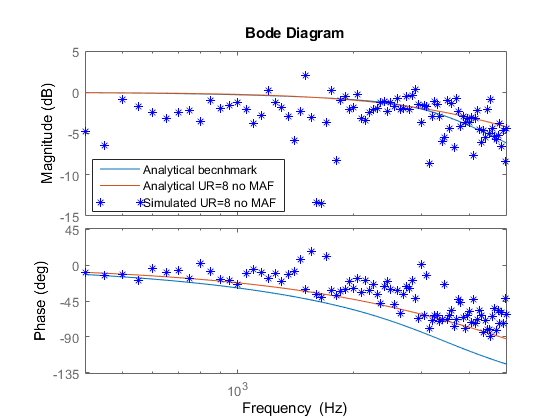
\includegraphics[width=0.95\linewidth]{figures/nasb_clfra.png}}
    \caption{Current loop in-phase condition for $N = 4, D_c = \frac{1}{4}$. The area tells the boundary phase-lag at the switching frequency, introduced by $G_{fb}(z)$, below which the in-phase operation begins.}
    \label{fig:N4InPhaseCondition}    
\end{figure}

It is concluded that current control loops can feature in-phase operation only if derivative gain is not used (P or PI controller). 
Therefore, the boundary phase-lag lines for the PI current loop are shown in Fig. \ref{fig:PIInPhaseCondition}, for $N \in \{4,6,8\}$. Due to the approximations used in the modulating waveform calculations, it was of interest to verify these boundary lines. The simulations were implemented in MATLAB/Simulink, for the control system described in Fig. \ref{fig:MSControl} and for a buck converter described in Table \ref{tab: Converter}, section V. The first verification was performed by implementing $G_{fb}(z)$ as in \eqref{eq:lpf}. These results are shown in Fig. \ref{fig:PIInPhaseCondition} using circular markers. The second verification was performed with a cascade of two low-pass filters, with a unique cut-off frequency. The second verification (marked using diamonds in Fig. \ref{fig:PIInPhaseCondition}) is useful to demonstrate that the in-phase condition for current loos is strongly correlated to the equivalent phase-lag at the switching frequency. These results show that the presented calculations are well-suited to predict the in-phase operation independently of the specific converter parameters, exact duty cycle or filter configuration.

\begin{figure}[t!]
    \centerline{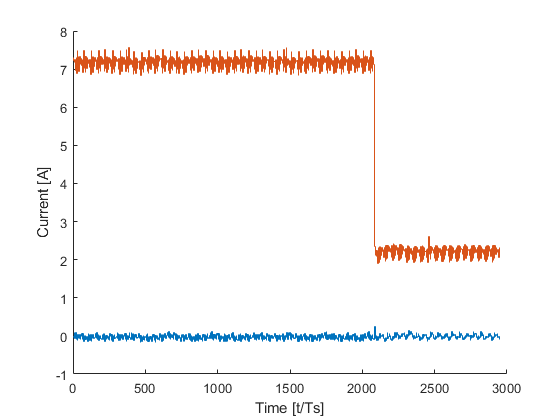
\includegraphics[width=0.95\linewidth]{figures/nasb_step.png}}
    \caption{Boundary lines for in-phase condition for current control loops with a PI controller for $N = 4$ and $D_c = \frac{1}{4}$, $N = 6$ and $D_c = \frac{1}{6}$, $N = 8$ and $D_c = \frac{1}{8}$. The in-phase condition is satisfied in regions below the boundary lines. Circular markers show the simulated result with $G_{fb}(z)$ in \eqref{eq:lpf}. Diamond markers show the simulated result for a cascade of two low-pass filters.}
    \label{fig:PIInPhaseCondition}
\end{figure}

\subsection{Modulator static transcharacteristic}
In , static transcharacteristic of the MS-PWM is given to show reduced gain zones of the modulator, which are related to counter-phase vertical intersections of $m_h(t)$ and $w(t)$. The same procedure is repeated in this paper, and the result for $N=6$ is shown in Fig. \ref{fig:TransCH}. The transcaracteristic is given for a current loop of the converter described in Table \ref{tab: Converter}, with a feedback filter configuration corresponding to experimentally verified case C in Table \ref{tab: Experimentals}.

\begin{figure}[t!]
    \centerline{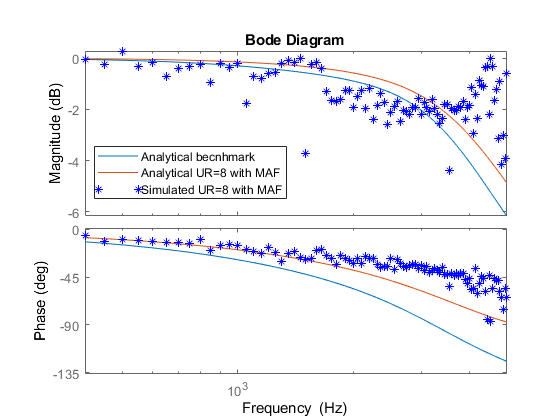
\includegraphics[width=0.95\linewidth]{figures/nasDif_clfra.png}}
    \caption{The modulator static transcharacteristic for $N=6$.}
    \label{fig:TransCH}    
\end{figure}

The transcharacteristic represents the average value of the modulating waveform $<m>$ that results in steady-state duty-cycle $D$. 
In Fig. \ref{fig:TransCH}, both counter-phase and in-phase effects are seen around $D = \frac{1}{3}$ and $D = \frac{2}{3}$. The counter-phase zone around $D = \frac{1}{3}$ occurs during down-count of the carrier and around $D = \frac{2}{3}$ for up-count of the carrier, and vice-versa for in-phase zones. The counter-phase affects the transcharacteristic by introducing reduced-gain zones, where $\frac{dD}{d<m>}\approx \frac{1}{2}$  . The in-phase jitter zones, filled with a dot pattern, represent parts of the transcharacteristic where steady-state can not be achieved. In zoomed window of Fig. \ref{fig:TransCH}, two required operating points are shown. The first one, $D(i_{L,r1})$, corresponds to the linear part of the transcharacteristic, hence, steady-state $D$ is found. The second one, $D(i_{L,r2})$, is located in the jitter zone and therefore it results in jitter amplification. A step response between these two operating points is tested in section V. The transcharacteristic in jitter zones is almost vertical, which is why they are referred to as "increased gain" zones. 

Note that the analytic procedure used to obtain the transcharacteristic can be used to exactly determine whether the "in-phase" regime occurs, for any specific converter topology or control stage.


\section{Simulation results}

This section shows simulation results for operating regime that feature the jitter amplification. The results are given for a current loop of a DC-DC buck converter, described in Table \ref{tab: Converter}. 

\begin{table}[h!]
			  \caption{Buck converter parameters}
              \label{tab: Converter}
              \centering
              \begin{tabular}{llll}
                           \midrule\midrule
        Converter parameters     & label           & value             & unit\\
        \midrule               
                  Input voltage   	& $V_{in}$      & 200    & V\\  
                  Inductance    & $L$      & 0.6    & mH\\
                  Capacitance    & $C$      & 30    & $\mathrm{\mu F}$\\
                  Output load resistor    & $R$      & 30    & \si{\ohm}\\
                  Switching frequency    & $f_{sw}$      & 20    & kHz\\
                  \midrule\midrule
        PI controller parameters & label           & value             & unit\\
                  \midrule
                  Proportional gain    & $k_p$      & 0.035    & $\mathrm{\frac{1}{A}}$\\
                  Integral gain    & $k_i$    & 131    & $\mathrm{\frac{1}{As}}$\\        
                  Crossover frequency    & $f_c$    & 2.5    & kHz\\                                                         
                  \midrule\midrule
              \end{tabular}
\end{table}

The simulations are organized in the following manner. The inductor current spectra are verified for a feedback path consisting of an anti-aliasing ALPF, and for three cases regarding the use of a DLPF: without DLPF (counter-phase regime without jittering, as a benchmark), with DLPF (in-phase regime with jittering), and with DLPF and anti-jittering algorithm. The feedback configuration is explained in detail in Section VI. The data is acquired with a rate of $500$ MS/s, and the window length is equal to $50$ ms.

For the manuscript brevity, the simulation results of inductor current spectra are shown only for $N = 4$ and average current equal to $3.25$ A. The presented regime features jittering on both up- and down-count of the carrier. The results are shown in Fig. \ref{fig:N4Simulations}. From the presented results, it is clear that the jittering causes very high effect on the inductor current, which is successfully prevented using the proposed algorithm. 

\begin{figure}[t!]
    \centerline{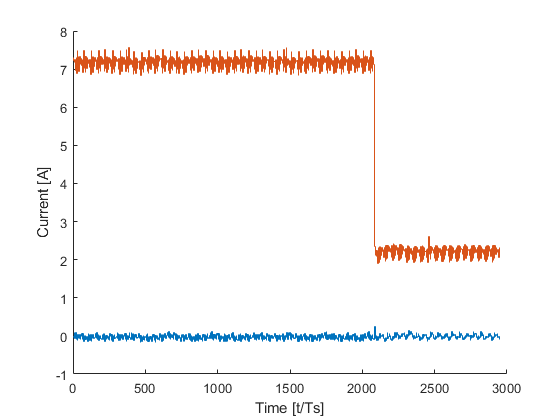
\includegraphics[width=0.95\linewidth]{figures/nasb_step.png}}
    \caption{Simulation results of inductor current spectra for $N = 4$.}
    \label{fig:N4Simulations} 
\end{figure}

The time-domain simulation results are provided for $N=6$ (for which the transcharacteristic is given in Fig. \ref{fig:TransCH}), in order to test the algorithm dynamic performance.
The step responses are tested from $i_{L,r1} = 4.43$ A (required duty cycle equal to $0.665$ - linear zone) to $i_{L,r1} = 4.51$ A (required duty cycle equal to $0.677$ - jitter zone). The results are given without (Fig. \ref{fig:step_simulation_sub1}) and with the proposed algorithm (Fig. \ref{fig:step_simulation_sub2}).

\begin{figure}[t!]
\centering
\begin{subfigure}{0.5\textwidth}
  \centering
  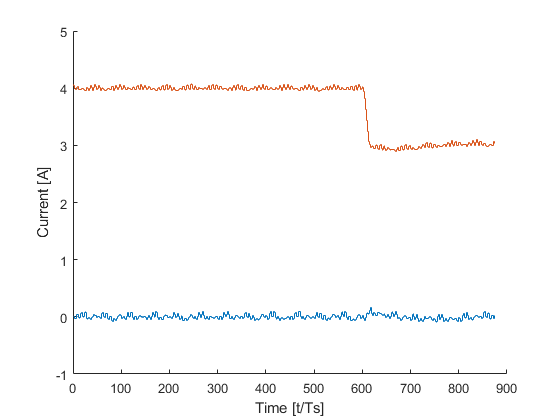
\includegraphics[width=0.95\linewidth, height = 45mm]{figures/nasDif_step_3Rs.png}
  \caption{}
  \label{fig:step_simulation_sub1}
\end{subfigure}\\
\begin{subfigure}{0.5\textwidth}
  \centering
  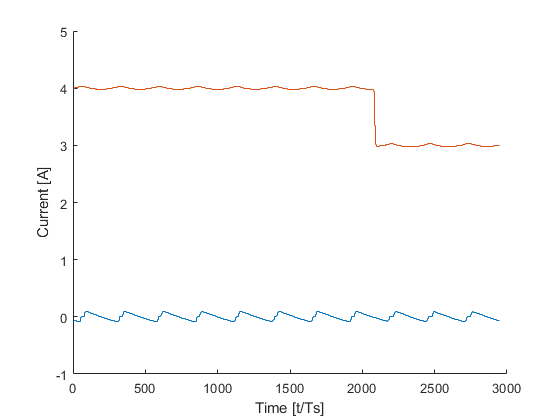
\includegraphics[width=0.95\linewidth, height = 45mm]{figures/nasDif_step_50Hz.png}
  \caption{}
  \label{fig:step_simulation_sub2}
\end{subfigure}\\
\caption{Simulation results of inductor current step responses for $N=6$, from linear to jitter zone: (a) without proposed algorithm; (b) with proposed algorithm.}
\label{fig:step_simulation}
\end{figure}
\noindent
From Fig. \ref{fig:step_simulation}, it can be seen that the operating point enters the jitter zone at approximately $t = 1.6$ ms. This causes a slight transient when the anti-jittering algorithm is used, as the blocking of the modulating waveform update begins after the first jitter is detected.

\begin{figure}[t!]
    \centerline{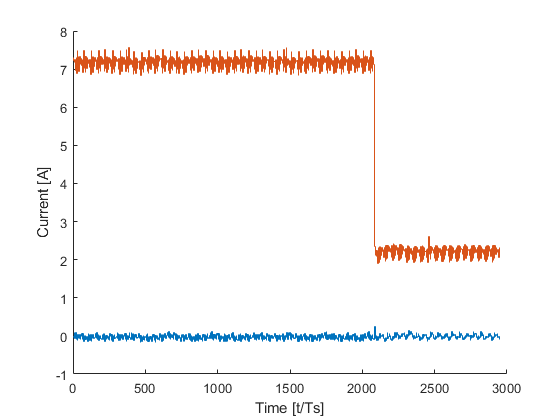
\includegraphics[width=0.95\linewidth]{figures/nasb_step.png}}
    \caption{Simulation results of relative reference tracking errors for $N=6$: (a) counter-phase operation; (b) in-phase operation without the proposed algorithm, and (c) in-phase operation with the proposed algorithm.}
    \label{fig:errorAVG}    
\end{figure}

In Fig. \ref{fig:errorAVG}, reference tracking errors for step responses shown in Fig. \ref{fig:step_simulation} are plotted in order to observe the algorithm impact on the loop dynamics. The error traces are plotted relative to the current reference, after using a moving average filter to remove the switching frequency components. It can be seen that the algorithm does not significantly impact the step response, and the error caused by blocking the modulating waveform is quickly compensated by the controller. In jitter zones, when the modulating waveform update is blocked once or twice per switching period, the small-signal DPWM dynamics are only slightly deteriorated, due to the reduced update rate. Furthermore, any large disturbance is compensated without delays due to the adaptive nature of the anti-jittering algorithm. 

\section{Experimental verification}
The experimental demonstration of the described jittering phenomenon and the verification of the proposed anti-jittering algorithm is shown in this section. The results are shown for a buck converter, described in Table \ref{tab: Converter}. A $2$ kW half-bridge hardware setup, which corresponds to the one shown in Fig. \ref{fig:MSControl}, is controlled using a digital signal processor from Texas Instruments C2000 series, TMS320F28379D. The results are given for multisampling factors $N \in \{4,6,8 \}$. The inductor current data is obtained using a current probe with $300$ kHz bandwidth and oscilloscope RIGOL MS05104. The modulating waveforms are extracted from Code Composer Studio, using arrays with $2000$ points. 
The experimental results are summarized in Table \ref{tab: Experimentals}.

\begin{table}[h!]
			  \caption{Summary of experimental results}
              \label{tab: Experimentals}
              \centering
              \begin{tabular}{llll}
				  \midrule\midrule
        		  Data information   								& label 					& value 			& unit 	\\
        		  \midrule
                  Data window length   									& $T_{data}$   				& $50$    			& ms	\\ 
                  Acquisition rate    									& $f_{acq}$      			& $500$    			& MS/s 	\\
                  ADC resolution										& $LSB$						& $9.76$			& mA	\\
                  Digital LPF cut-off frequency							& $f_{c,DLPF}$			& $20$				& kHz 	\\
                  Analog LPF cut-off frequency							& $f_{c,ALPF}$			& $30$				& kHz 	\\                
                  \midrule\midrule
        		  Case A: $N = 4$, up-count   											& label 					& value 			& unit \\
        		  \midrule
                  Inductor current   									& $i_{L}$      				& $3.12$    			& A\\ 
                  Duty cycle    										& $D$      					& $0.48$    		& /\\
                  Duty cycle variance   								& $\sigma ^2 _D $    		& $3.78 \cdot 10^{-6}$   & /\\
				  Calculated duty cycle variance \eqref{eq:variance_D}	& $\sigma ^2 _D$      		& $3.64 \cdot 10^{-6}$   & /\\                  
				  Duty cycle variance with anti-jittering    			& $\sigma ^2 _D$      		& $3.65 \cdot 10^{-7}$    & /\\
                  Duty cycle variance without DLPF    					& $\sigma ^2 _D$      		& $8 \cdot 10^{-7}$    & /\\
                  Feedback filter configuration							& \multicolumn{3}{l}{Digital LPF}\\
                  \midrule\midrule
        		  Case B: $N = 4$, up- and down-count   											& label 					& value 			& unit \\
        		  \midrule
                  Inductor current   									& $i_{L}$      				& $3.25$    			& A\\ 
                  Duty cycle    										& $D$      					& $0.5$    		& /\\
                  Duty cycle variance   								& $\sigma ^2 _D $    		& $3.9 \cdot 10^{-5}$   & /\\
				  Calculated duty cycle variance \eqref{eq:variance_D}	& $\sigma ^2 _D$      		& $3.6 \cdot 10^{-5}$   & /\\                  
				  Duty cycle variance with anti-jittering    			& $\sigma ^2 _D$      		& $3.4 \cdot 10^{-7}$    & /\\
                  Duty cycle variance without DLPF    					& $\sigma ^2 _D$      		& $8 \cdot 10^{-7}$    & /\\
                  Feedback filter configuration							& \multicolumn{3}{l}{Digital and Analog LPF}\\
                  \midrule\midrule        
        		  Case C: $N = 6$, up-count 											& label 					& value 			& unit \\
        		  \midrule
                  Inductor current   									& $i_{L}$      				& $2.13$    			& A\\ 
                  Duty cycle    										& $D$      					& $0.33$    		& /\\
                  Duty cycle variance   								& $\sigma ^2 _D $    		& $7.5 \cdot 10^{-6}$   & /\\
				  Calculated duty cycle variance \eqref{eq:variance_D}	& $\sigma ^2 _D$      		& $4.7 \cdot 10^{-6}$   & /\\                  
				  Duty cycle variance with anti-jittering    			& $\sigma ^2 _D$      		& $4.25 \cdot 10^{-7}$    & /\\
                  Duty cycle variance without DLPF    					& $\sigma ^2 _D$      		& $4.35 \cdot 10^{-7}$    & /\\
                  Feedback filter configuration							& \multicolumn{3}{l}{Digital and Analog LPF}\\
                  \midrule\midrule    
                  Case D: $N = 8$, up-count  											& label 					& value 			& unit \\
        		  \midrule
                  Inductor current   									& $i_{L}$      				& $1.61$    			& A\\ 
                  Duty cycle    										& $D$      					& $0.246$    		& /\\
                  Duty cycle variance   								& $\sigma ^2 _D $    		& $4 \cdot 10^{-6}$   & /\\
				  Calculated duty cycle variance \eqref{eq:variance_D}	& $\sigma ^2 _D$      		& $1.9 \cdot 10^{-6}$   & /\\                  
				  Duty cycle variance with anti-jittering    			& $\sigma ^2 _D$      		& $1.97 \cdot 10^{-7}$    & /\\
                  Duty cycle variance without DLPF    					& $\sigma ^2 _D$      		& $8.2 \cdot 10^{-7}$    & /\\
                  Feedback filter configuration							& \multicolumn{3}{l}{Digital and Analog LPF}\\
                  \midrule\midrule       
              \end{tabular}
\end{table}

The controller is tuned to obtain a crossover frequency $f_{c} = \frac{1}{8} f_{sw} = 2.5$ kHz. 
The feedback path consists of an ALPF with cut-off frequency equal to $30$ kHz, and a DLPF with cut-off frequency equal to the switching frequency of the converter. This kind of cascaded filter configuration is common in practice, especially for multisampled control. The ALPF is used to suppress the aliasing effect. It introduces $34$ degrees phase lag at the switching frequency and $4.7$ degrees phase lag at the crossover frequency. The DLPF is introduced to suppress the nonlinearity of the DPWM, which is present in MS-PWM control systems. It introduces $45$ degrees phase lag at the switching frequency and $7$ degrees phase lag at the crossover frequency. The combined phase lag of the feedback filter cascade is equal to $79$ degrees at the switching frequency. Based on Fig. \ref{fig:PIInPhaseCondition}, this filter cascade enables the in-phase regime for all tested values of the multisampling factor. The results with this filter configuration are shown in Figs. \ref{fig:N430kHz} - \ref{fig:adaptive_algo}. The DLPF on its own is enough to enable the in-phase regime for $N = 4$, hence this regime is tested as well and the results are shown in Fig. \ref{fig:N4100kHz}.
The experimental results are organized to show three operating conditions, for each multisampling factor. The current references are chosen to feature jitter amplification when the DLPF is employed. When the DLPF is bypassed, the operating mode is counter-phase, which is used as a benchmark without jittering. Finally, the results are shown for the operating mode when the DLPF is turned on and the anti-jittering algorithm is employed.
The results are shown as spectra of the inductor current, which clearly demonstrate the negative impact of jittering. Furthermore, modulating waveforms are extracted from the DSP, and used to calculate variances of applied duty cycles. These variances are compared with the analytical values, calculated using \eqref{eq:variance_D}. For the calculations, the difference between critical modulating segments is averaged over the available array. It should be noted that all measurements were repeated several times, with consistent conclusions.

The first result, shown in Fig. \ref{fig:N4100kHz} is given for the case of $N=4$, without the ALPF in the feedback (case A). The regime corresponds to jittering due to the intersection with the carrier during up-count mode. It can be seen that the calculated duty cycle variance matches very well with the experimentally obtained result. The variance is approximately $10$ times higher in the jittering regime compared to the regime with anti-jittering algorithm.

\begin{figure}[t!]
\centering
\begin{subfigure}{0.5\textwidth}
  \centering
  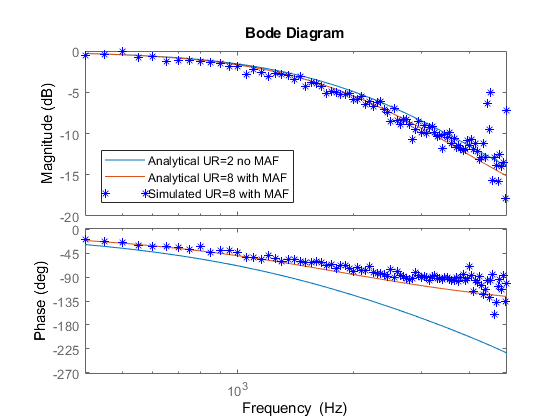
\includegraphics[width=0.95\linewidth, height = 45mm]{figures/nas_clfra.png}
  \caption{}
  \label{fig:N4100kHz_sub1}
\end{subfigure}\\
\begin{subfigure}{0.5\textwidth}
  \centering
  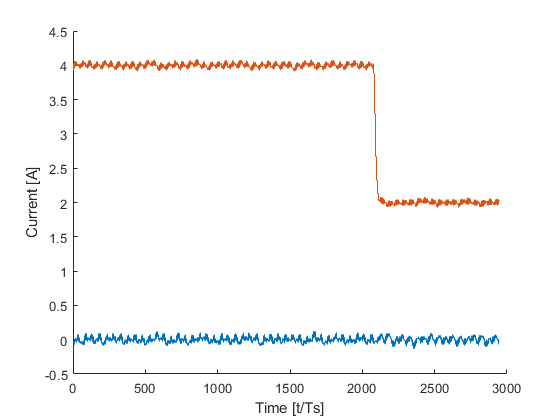
\includegraphics[width=0.95\linewidth, height = 45mm]{figures/nas_step.png}
  \caption{}
  \label{fig:N4100kHz_sub2}
\end{subfigure}\\
\caption{The results for case A: (a) Spectra of the inductor current; (b) Variance of the applied duty cycle.}
\label{fig:N4100kHz}
\end{figure}

\begin{figure}[t!]
\centering
\begin{subfigure}{0.5\textwidth}
  \centering
  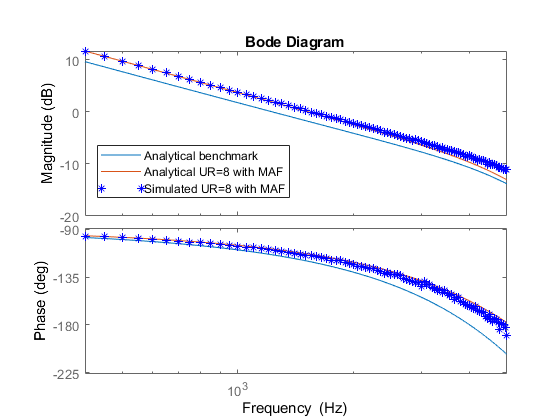
\includegraphics[width=0.95\linewidth, height = 45mm]{figures/nasDif_ollfra.png}
  \caption{}
  \label{fig:N430kHz_sub1}
\end{subfigure}\\
\begin{subfigure}{0.5\textwidth}
  \centering
  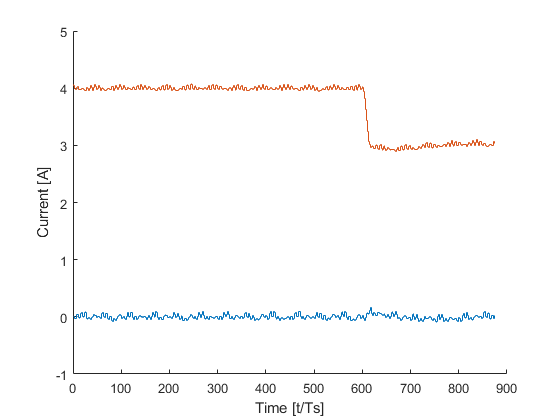
\includegraphics[width=0.95\linewidth, height = 45mm]{figures/nasDif_step_3Rs.png}
  \caption{}
  \label{fig:N430kHz_sub2}
\end{subfigure}\\
\caption{The results for case B: (a) Spectra of the inductor current; (b) Variance of the applied duty cycle.}
\label{fig:N430kHz}
\end{figure}

\noindent
Subsequent results, shown in Figs. \ref{fig:N430kHz} - \ref{fig:adaptive_algo} are given for the cascaded filter configuration that employs both ALPF and DLPF in the feedback. 
The time-domain waveform, for $N = 4$ and jittering during both up- and down-count of the carrier (case B), can be seen in the active contents submitted with this paper. The contents feature two videos of oscilloscope screen named $jittering\_ caseB.mp4$ and $jittering\_ caseB\_ zoom.mp4$ that are given to demonstrate the presented jitter amplification and anti-jittering algorithm operation.
For the same regime, spectral results and duty cycle variances are shown in Fig. \ref{fig:N430kHz}. It should be noted that the duty cycle variance for this case is equal to sum of variances from \eqref{eq:variance_D} for both pairs of critical modulating segments. This case shows extremely high difference between the duty cycle variances for cases with and without jittering.
This regime corresponds to the simulation result shown in Fig. \ref{fig:N4Simulations}. An excellent match between these two results is a good sign that the analytic reasoning behind the phenomenon is consistent with the experimental behavior. The spectral waveform of $i_L$ during jittering shows emphasized peaks around $5$ kHz, $10$ kHz and $15$ kHz, which highlights the deterministic nature of the nonlinear phenomenon.

Fig. \ref{fig:N630kHz} shows results for the case of $N=6$ and up-count jittering (case C). There is a slight error between the calculated and applied duty cycle variance for the jittering case. The applied duty cycle variance is approximately $17$ times higher for the regime with jittering compared to the regime with anti-jittering algorithm. Fig. \ref{fig:N830kHz} shows results for the case of $N=8$ and up-count jittering (case D). Again, there is a slight error between the calculated and applied duty cycle variance for the jittering case. The applied duty cycle variance is approximately $20$ times higher for the regime with jittering compared to the regime with anti-jittering algorithm.

\begin{figure}[t!]
\centering
\begin{subfigure}{0.5\textwidth}
  \centering
  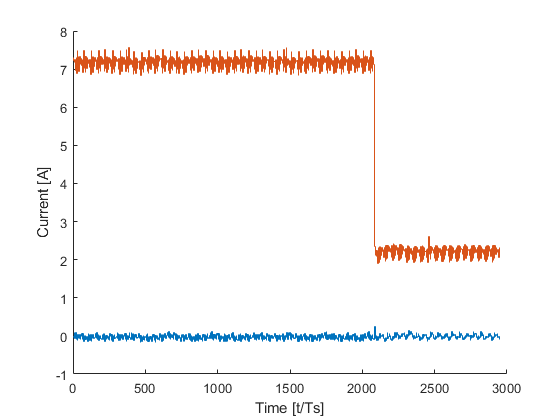
\includegraphics[width=0.95\linewidth, height = 45mm]{figures/nasb_step.png}
  \caption{}
  \label{fig:N630kHz_sub1}
\end{subfigure}\\
\begin{subfigure}{0.5\textwidth}
  \centering
  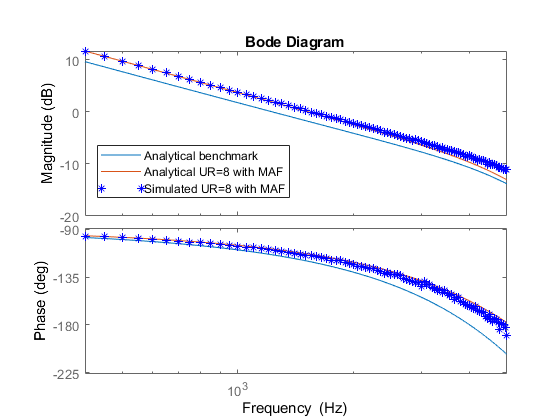
\includegraphics[width=0.95\linewidth, height = 45mm]{figures/nasDif_ollfra.png}
  \caption{}
  \label{fig:N630kHz_sub2}
\end{subfigure}\\
\caption{The results for case C: (a) Spectra of the inductor current; (b) Variance of the applied duty cycle.}
\label{fig:N630kHz}
\end{figure}

\begin{figure}[t!]
\centering
\begin{subfigure}{0.5\textwidth}
  \centering
  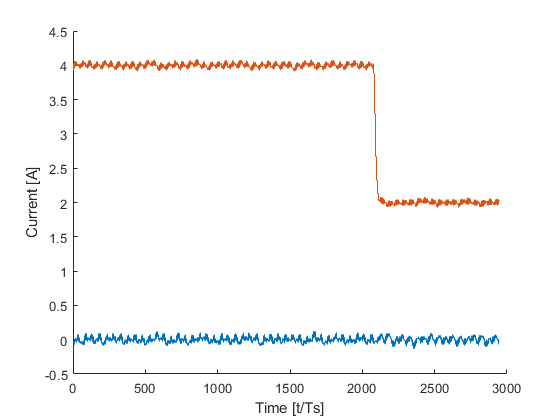
\includegraphics[width=0.95\linewidth, height = 45mm]{figures/nas_step.png}
  \caption{}
  \label{fig:N830kHz_sub1}
\end{subfigure}\\
\begin{subfigure}{0.5\textwidth}
  \centering
  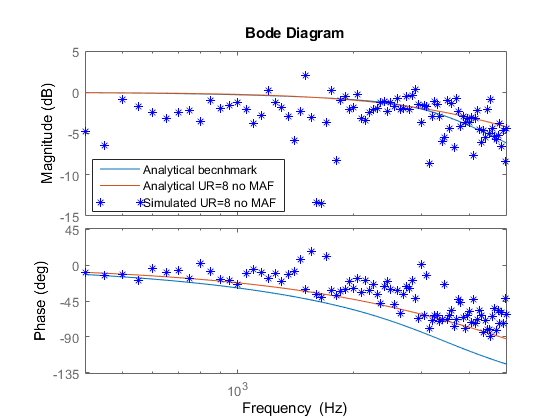
\includegraphics[width=0.95\linewidth, height = 45mm]{figures/nasb_clfra.png}
  \caption{}
  \label{fig:N830kHz_sub2}
\end{subfigure}\\
\caption{The results for case D: (a) Spectra of the inductor current; (b) Variance of the applied duty cycle.}
\label{fig:N830kHz}
\end{figure}

\noindent
An important feature of the anti-jittering algorithm is to detect large-signal disturbances, and prevent the blocking of the modulating waveform update. Fig. \ref{fig:adaptive_algo} is given to demonstrate that the algorithm allows detection of large-signal disturbances and offers an unimpaired response to a reference step change. The result is given for case B. This example demonstrates the effectiveness of the proposed adaptive limits, which are used to determine whether the modulating waveform update should be allowed or not. The algorithm parameters are calculated based on converter parameters, which indicates that the tuning can be universally effective for each converter design.

\begin{figure}[t!]
    \centerline{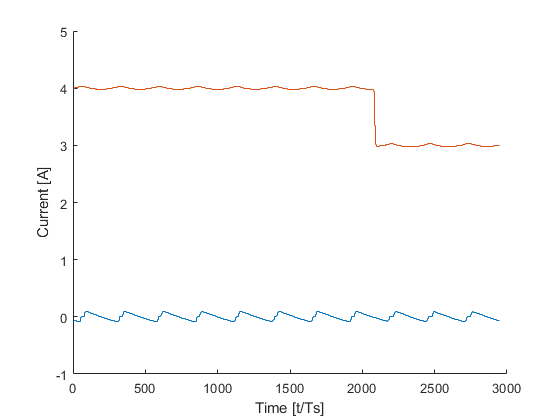
\includegraphics[width=0.95\linewidth]{figures/nasDif_step_50Hz.png}}
    \caption{Algorithm operation for $i_{L,r}$ step change from $3.25$ A to $4$ A, for case B. The $m_h(t)$ represents the modulating waveform before the algorithm; $m_{out}$ represents the applied modulating waveform.}
	\label{fig:adaptive_algo}
\end{figure}

From the experimental results, it is clear that the jittering impact on the inductor current can be very high. The results also clearly demonstrate that the proposed anti-jittering algorithm is capable of canceling the jittering phenomenon. The experimental results show that the presented statistical approach is well-suited to describe this phenomenon, as the estimation of the applied duty cycle variance shows good match with the obtained values. It is important to note that the jittering effect has stronger impact for lower multisampling factors, which is due to the higher discontinuity of the modulating waveform. For current loops, higher phase lag also increases the jittering effect as the in-phase operating mode is more emphasized, which is seen in results with both filters in the feedback.


\section{Conclusion}
This paper has presented a newly discovered phenomenon, related to MS-PWM control. Strong jittering of the duty cycle is enabled by the discontinuity of the modulating waveform and in-phase relation between the modulating waveform and the carrier. The controller/feedback configuration, which enables jittering is analytically derived for inductor current loops. The impact of jittering on the applied duty cycle is statistically modelled. Jittering regimes are tested in simulations and experimentally, showing a good match with the analytical considerations.
The jittering is attenuated by decreasing the modulating waveform discontinuity, which is why choosing higher multisampling factors is recommended. Additionally, an algorithm that prevents jittering is developed and tested, with emphasis on its dynamic performance. 

\ifCLASSOPTIONcaptionsoff
  \newpage
\fi

\bibliographystyle{IEEEtran}
% argument is your BibTeX string definitions and bibliography database(s)
\bibliography{IEEEabrv,bib/mybibliography.bib}

\end{document}



